\documentclass{article}
\usepackage[utf8]{inputenc}
\usepackage{listings}
\usepackage{geometry,tikz,pgfplots,multicol,relsize,enumitem}
\usepackage{mathtools}
\usepackage{graphicx}
\usepackage{amsfonts} 
\usepackage{listings}
\usepackage{amsmath}
\geometry{a4paper,bottom=1.5cm}


\title{Progetto Algoritmi e Strutture dati}
\author{Petreti Andrea\\\small Matricola 272822}
\date{25 Giugno 2016}
\begin{document}


\maketitle
\thispagestyle{empty}

\newpage 

\renewcommand{\contentsname}{Indice}

\tableofcontents

\newpage

\section{Introduzione}
Si vuole implementare un noto protocollo di messaggistica chiamato MQTT (Message Queue Telemetry Transport). MQTT è un protocollo M2M, ovvero machine to machine, viene applicato soprattuto al nuovo settore IoT. In particolare è stato progettato per avere un'impatto basso sia a livello di risorse computazioni richieste, sia a livello di occupaazione di banda; basato sul pattern Publish/Subscribe prevede due componenti:
\begin{itemize}
	\item Message Broker
	\item Client MQTT
\end{itemize}
I client MQTT possono iscriversi ad una certa parola chiave detta "Topic", per poi ricevere successivamente dal Broker solo i messaggi che altri Client hanno inviato sullo stesso Topic. Il Broker, similmente all'archiettura Client-Server, svolge il ruolo di ``Server", e come si può intuire dal nome, si occupa di ricevere e smistare i vari messaggi ai vari destinatari, nonchè di mantenere la lista di Topic al quale ogni Client si è iscritto.

\begin{figure}[htbp]
	\centerline{
		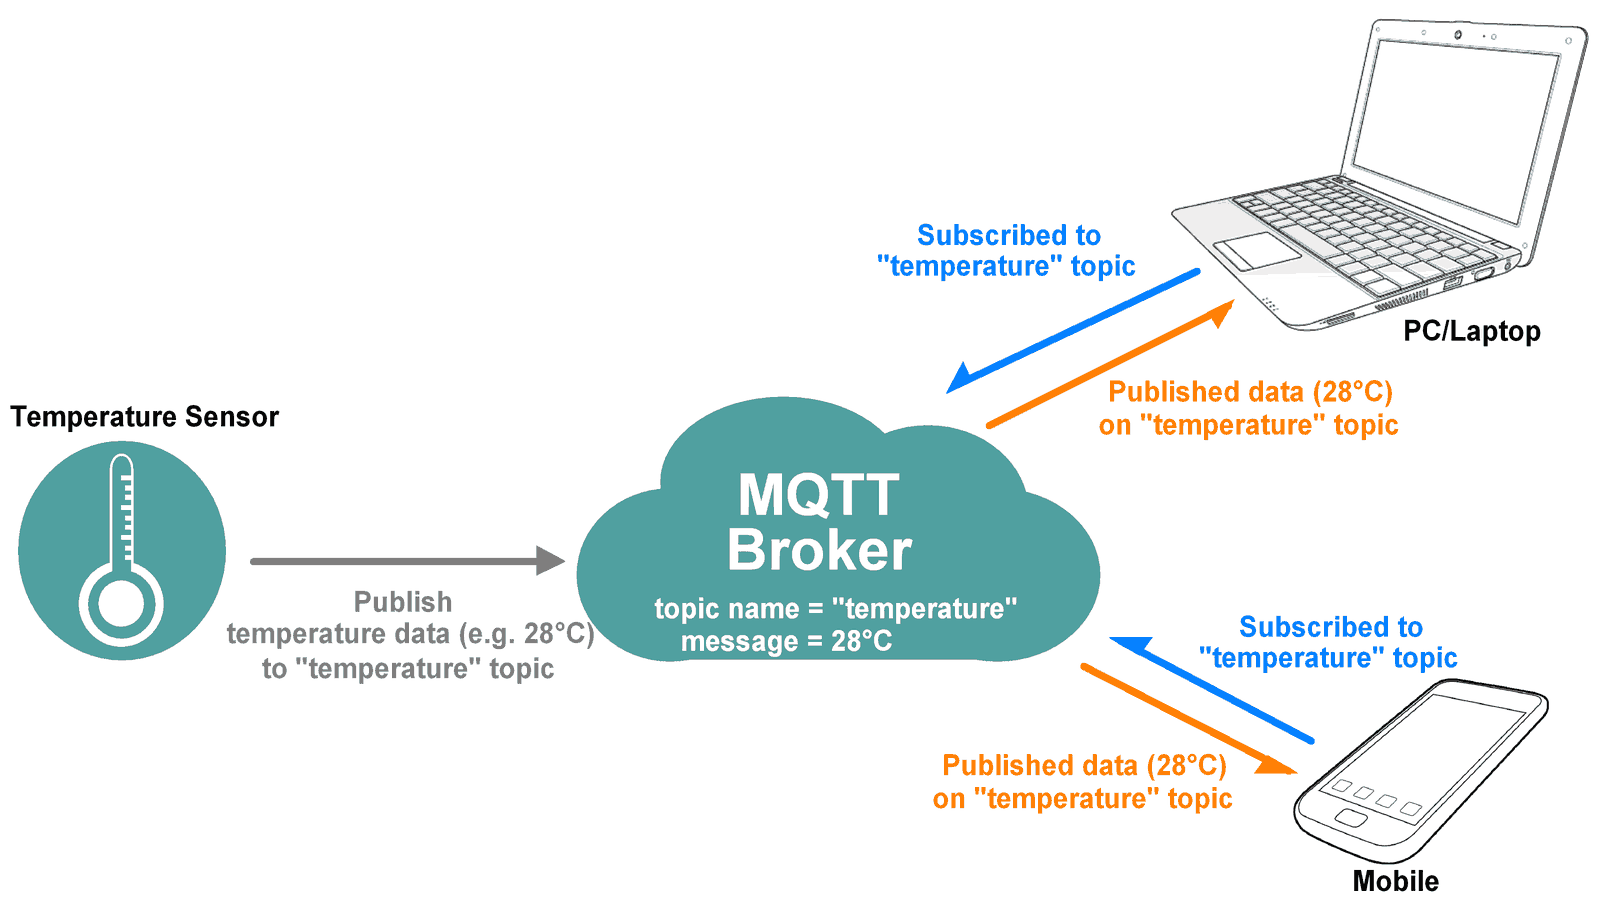
\includegraphics[scale=0.2]{immagini/broker_client_img.png}
	}
\end{figure}

L'immagine mostra un'esempio concreto, abbiamo un sensore di temperatura, che periodicamente invia ``Pubblica" la temperatura registrata, svolgento quindi il ruolo da Cliente che pubblica informazioni al Broker. Mentre il laptop e lo smartphone, si sono iscritti al Topic ``Temperature", e quindi ricevono i dati misurati dal sensore per mezzo del Broker.\\\\
MQTT però ha altre peculiarità, abbiamo detto che si presta bene in situazioni in cui abbiamo banda limitata, questo perchè ogni pacchetto del protocollo MQTT, prevede solo 2 byte di header fisso, inoltre minimizza anche gli scambi di messaggi, mettendo a disposizione tre livelli di servizio, che vengono anche chiamati Qos (Quality of Service).

\begin{figure}[htbp]
	\centerline{
		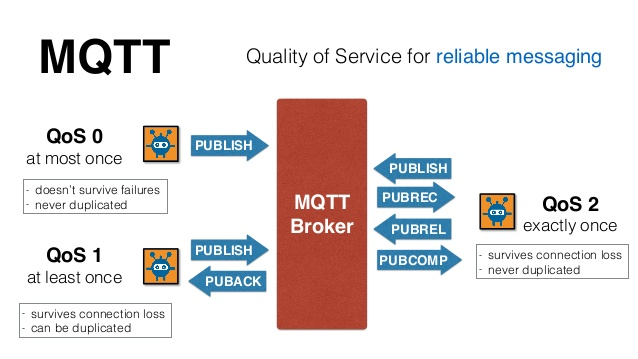
\includegraphics[scale=0.4]{immagini/mqtt_qos.jpg}
	}
\end{figure}

\begin{itemize}
	\item Qos 0 o ``at most once" o ``fire and forget", non da alcuna sicurezza dal punto di vista della mancata consegna o della duplicazione di messaggi, quindi se il messaggio viene perso o duplicato, il Client che ha inviato quel messaggio non può saperlo. Utilizzato nel caso in cui le informazioni non sono necessariamente importanti o nel caso in cui non ci interssa di ricevere messaggi duplicati.
	\item Qos 1 o ``at least once", viene assicurato l'arrivo dei messaggi al Broker, in quanto lui invierà un Ack di conferma, ma possono comunque verificarsi dei casi in cui il messaggio viene duplicato.
	\item Qos 2 o ``exactly once", ci assicura che il messaggio venga consegnato una sola volta e senza duplicazioni, ma l'invio di un message con questo tipo di servizio, aumenta ovviamente l'overhead, in quanto sono richiesti ben 3 Ack successevi da parte del Broker e da parte del Client.
\end{itemize}

MQTT supporta anche un minimo grado di sicurezza, permettendo l'invio nella fase di connessione di un'username e di una password, che poi il Broker dovrà valutare e garantire o meno la connessione, ovviamente in questo caso è necessario utilizzare un livello di transporto come TLS/SSL, oppure criptare e decriptare prima dell'invio e alla ricezione, per evitare che username e password possano essere letti da un'attacco man in the middle.


\section{Composizione Pacchetto MQTT}
Ogni pacchetto MQTT, come detto precedentemente ha un header fisso di 2 byte. Il primo di questi identifica la tipologia del pacchetto, e vari flag.
\begin{itemize}
	\item 4 bit per la tipologia del pacchetto tra cui: Connect, ConnAck, Publish, Subscribe, PubAck, PubRel, PubRec, PubComp, SubAck, Unsubscribe, UnsubAck, Disconnect, PingReq, PingResp.
	\item 1 bit per il flag di duplicazione del messaggio.
	\item 2 bit per la Qos, ovvero al Quality of Service.
	\item 1 bit per il flag Retain, di cui parlero nella sezione dedicata alla pubblicazione di un messaggio.

\end{itemize}Il secondo byte invece contiene la lunghezza della restante parte del pacchetto (payload), che varia a seconda della tipologia.

\section{Funzioni Principali MQTT}

\subsection{Connessione}
La connessione al Broker avviene tramite l'invio di un pacchetto di connessione (Connect), il quale contiene molte informazioni tra cui:

\begin{itemize}
	\item 
\end{itemize}

\subsection{Sessione}


\subsection{Pubblicazione}
La pubblicazione di un messaggio verso il Broker, avviene inviado ad esso un pacchetto MQTT (Publish Packet), che contiene:
\begin{itemize}
	\item Un Flag Retain, per indicare se quel messaggio deve essere salvato dal broker in maniera persistente ed inviato ai Client che si connetteranno e sottoiscriveranno successivamente allo stesso topic del messaggio.
	\item QOS, ovvero la qualità del servizio con la quale si vuole pubblicare quel messaggio al Broker. Qos può valore 0, 1 o 2, ed il Broker risponderà in maniera diversa a seconda della Qos. 
	\item Topic, ovvero la parola chiave, che identifica il canale in cui il messaggio verrà pubblicato.
	\item Messaggio, ovvero ciò che si vuole effettivamente pubblicare, come ad esempio un valore di temperatura, un messaggio testutale, ecc...
\end{itemize}
Il Broker dovrà invece:
\begin{itemize}
	\item Controllare quali Client sono sottoscritti allo stesso Topic, ed inviare loro il messaggio ricevuto, utilizzando come Qos il minimo tra la Qos del messaggio ricevuto e la Qos che i sottoscrittori hanno richiesto al momento della sottoscrizione.
	\item Salvare il messaggio in maniera permanente ed inviarlo (pubblicarlo) verso i Client che si iscriveranno anche in futuro al Topic del messaggio, se il Flag di retain è impostato.
	\item Inviare un PUBACK verso il Client che effettua la pubblicazione, se la Qos è uguale ad 1.
	\item Inviare un PUBREC verso il Client che effettua la pubblicazione, attendere che quest'ultimo risponda con un PUBREL, e concludere con l'invio di un PUBCOMP, se la Qos è uguale a 2.
\end{itemize}

\subsection{Sottoscrizione}
La richiesta di sottscrizione da parte del Client, avviene inviado al Broker un pacchetto MQTT, chiamato Subscribe Packet, che contiene:
\begin{itemize}
	\item Il classico header fisso, ma con Qos pari ad 1, poichè la sottscrizione prevede un ACK da parte del Broker.
	\item Topic al quale ci si vuole abbonare.
	\item Qos associata al Topic, per indicare che si vogliono ricevere messaggi dal Broker su quel Topic, con una certa Qos.
\end{itemize}
Il Broker all'arrivo di una richiesta di sottoscrizione dovrà:
\begin{itemize}
	\item Inviare un ACK verso il client, ovvero un paccheto del tipo PUBACK, nel quale deve specificare quale Qos il broker può garantire per il Topic richiesto dal Client.
	\item Inviare al Client stesso, se ci sono, i messaggi retain che il Broker aveva salvato per quel determinato Topic.
\end{itemize}
Inoltre il Client ha la possibilità di rimuovere la sottoscrizione ad un certo Topic, inviato un pacchetto ``Unsubscribe", il quale oltre ad avere un intestazione fissa con Qos 1, perchè anche esso prevede un Ack di ritorno, ovvero il UnsubAck, ha come payload il Topic che si vuole rimuovere.

\subsection{Keep Alive}
MQTT prevede un'meccanismo per stabilire se le due parti, ovvero Broker e Client, sono tra loro effettivamente connessi, utilizzando due tipologie di pacchetti: PingReq e PingResp. Al momento della connessione il Client specifica un certo tempo di keep alive al Broker. Quindi entrambi le parti avviano un timer, che viene azzerato ogni volta che arriva un pacchetto.\\
Quando il timer del Client raggiunge il tempo di keep alive, invia una richiesta di Ping, tramite un pacchetto di PingReq al Broker, il quale dovrà rispondere con pacchetto PingResp, se il Client riceve questa risposta entro il tempo di keep alive, la connessione continua, altrimenti viene interotta in quanto si ritiene che il Broker sia offline.\\
Il Broker, invece, quando il suo timer raggiunge il tempo di keep alive, la connessione con il Client viene automaticamente chiusa.\\

\textbf{N.B.} Ovviamente è importante che entrambi impostino una soglia in eccesso e in difetto per il keep alive, in modo tale da considere anche eventuali ritardi dovuti al traffico sulla rete. Ad esempio il Broker imposterà una soglia in eccesso per attendere leggermente oltre il tempo di keep alive, che il client invii almeno un'messaggio prima di chiudere la connessione. Mentre il cliente imposterà una soglia in difetto, per inviare un pacchetto di PingReq, prima del raggiungimento effetivo del tempo di keep alive.


\end{document}